\begin{figure}[H]
\centering 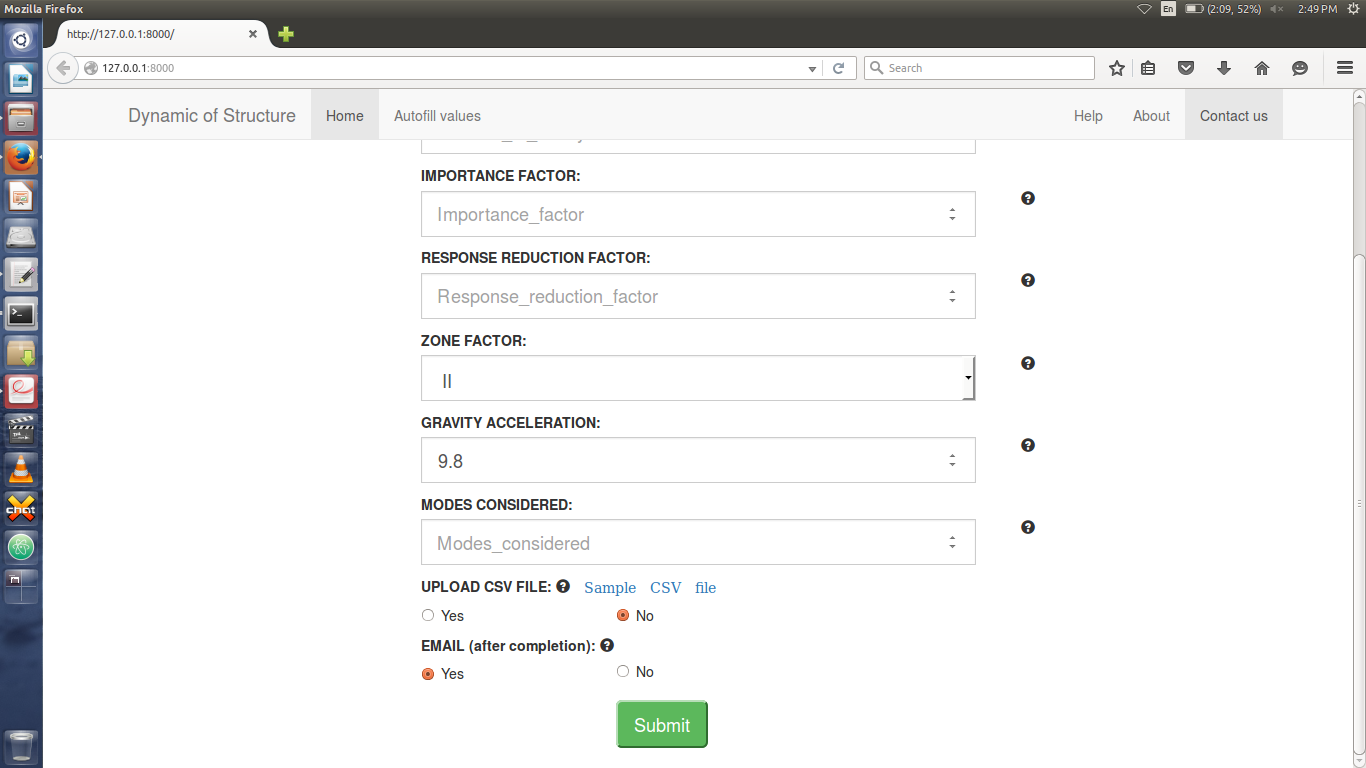
\includegraphics[scale=0.32]{images/output/1.png}
\caption{Home page of DoS}
\end{figure}
\begin{figure}[H]
\centering 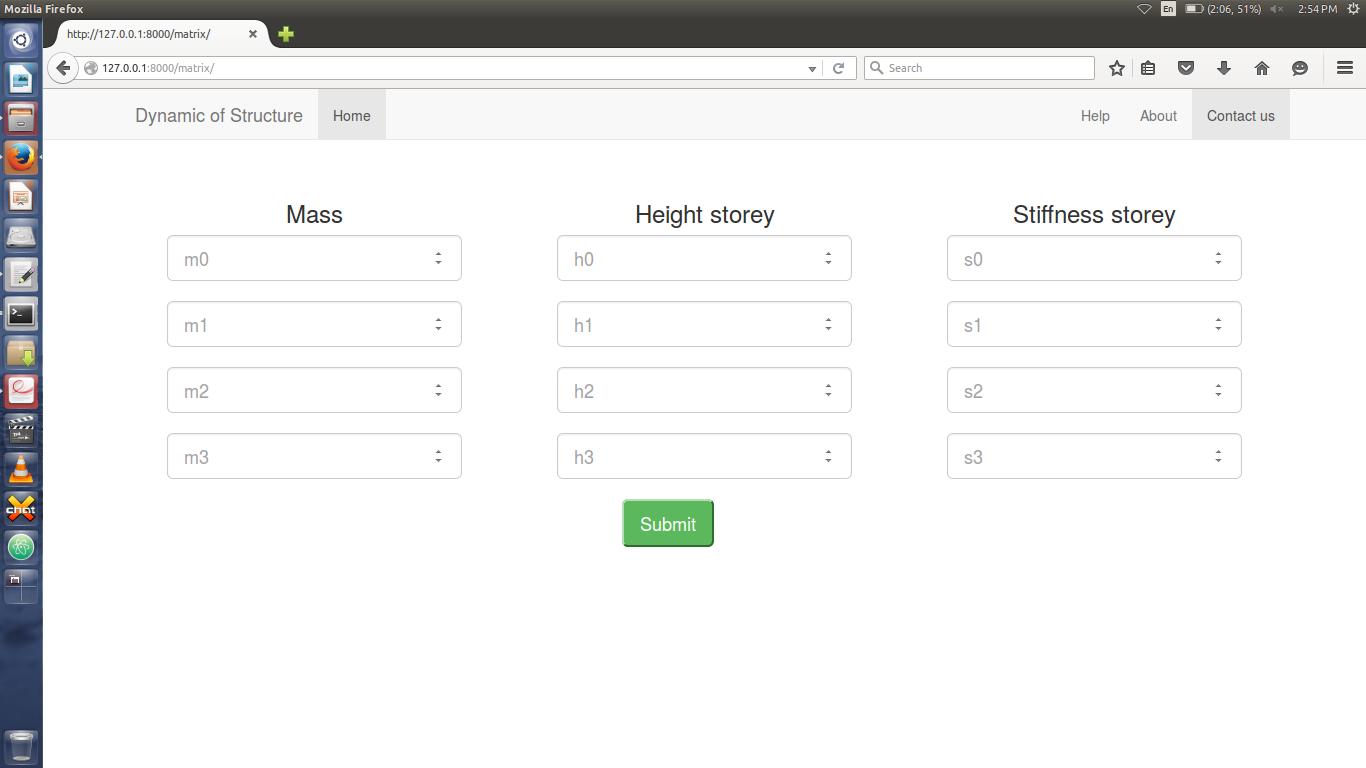
\includegraphics[scale=0.32]{images/output/2.png}
\caption{Matrix.html for manually filling values}
\end{figure}
\newpage
\begin{figure}[H]
\centering 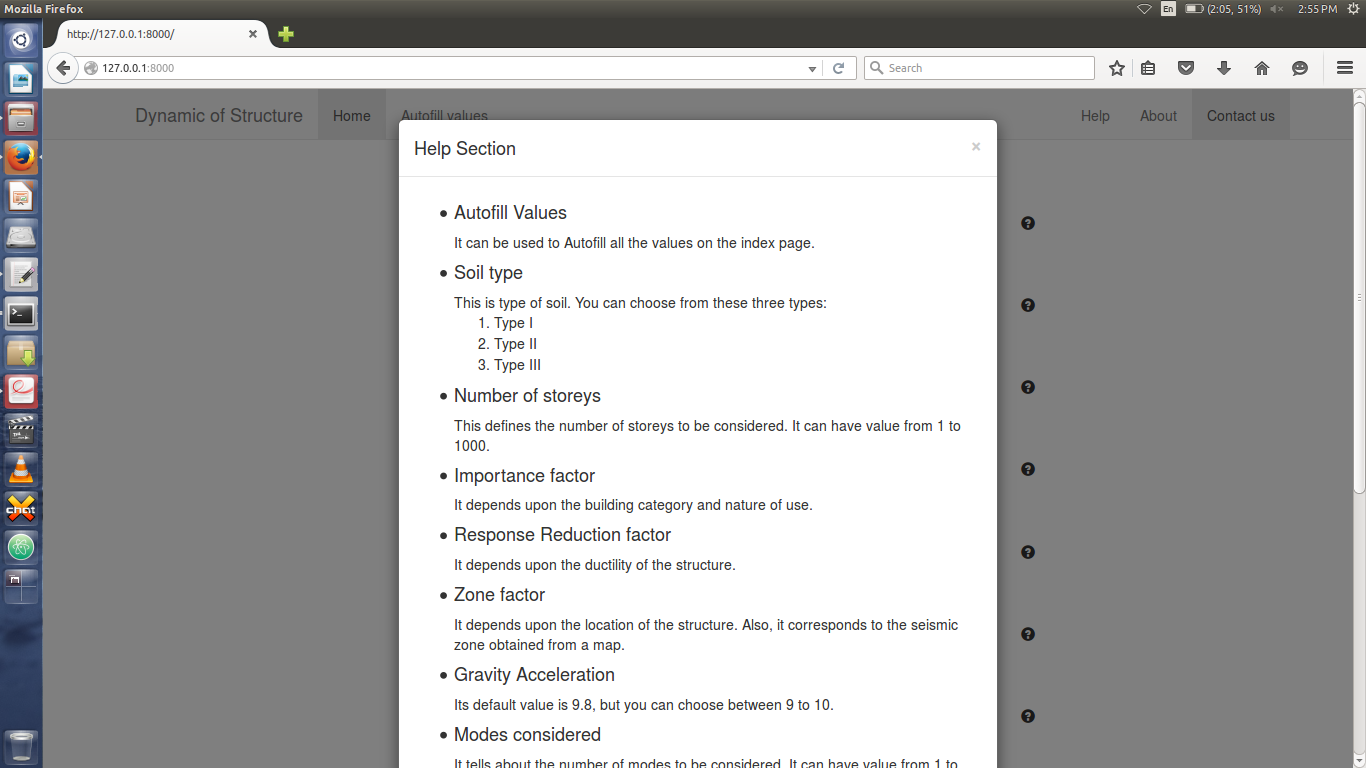
\includegraphics[scale=0.31]{images/output/3.png}
\caption{Help section in Home page}
\end{figure}
\begin{figure}[H]
\centering 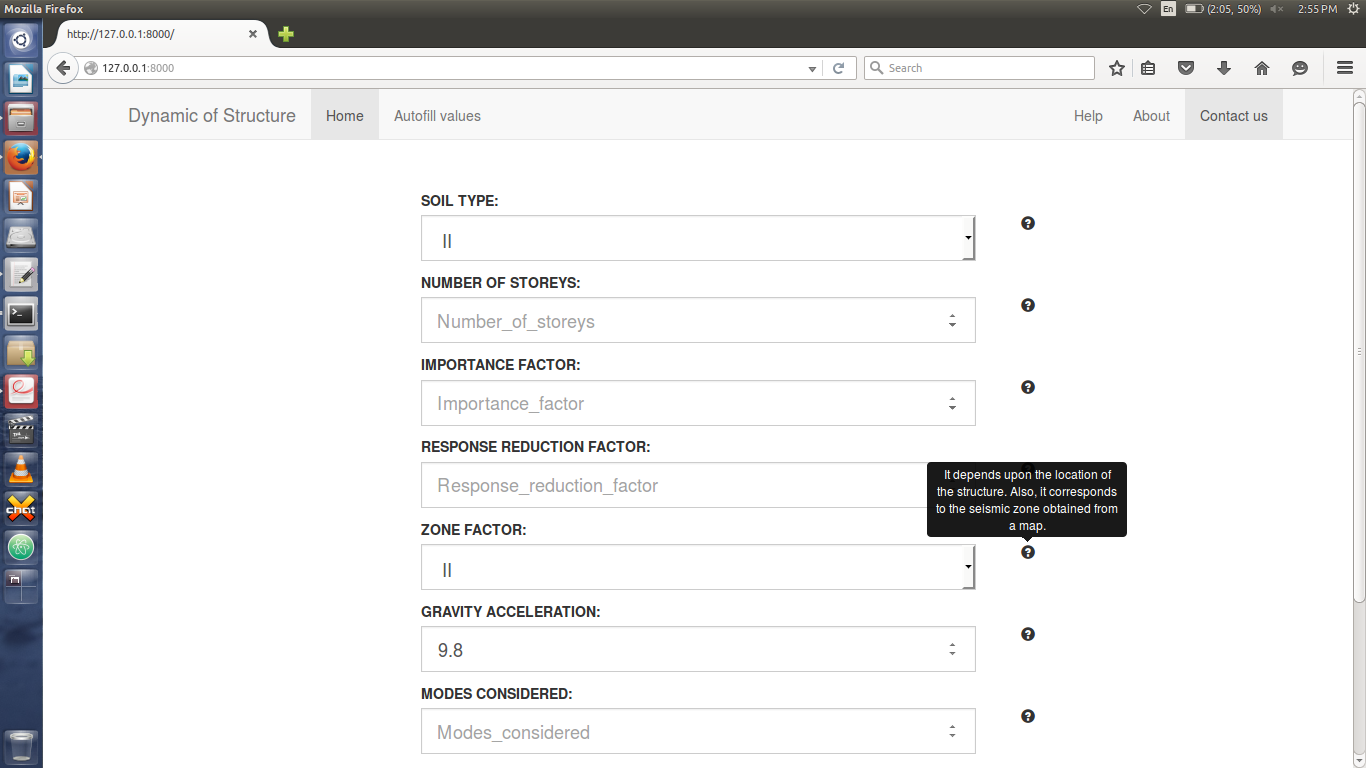
\includegraphics[scale=0.31]{images/output/4.png}
\caption{Local help option}
\end{figure}
\newpage
\begin{figure}[H]
\centering 
\includegraphics[scale=0.31]{images/output/6.png}
\caption{First page of PDF generated by DoS}
\end{figure}
\begin{figure}[H]
\centering 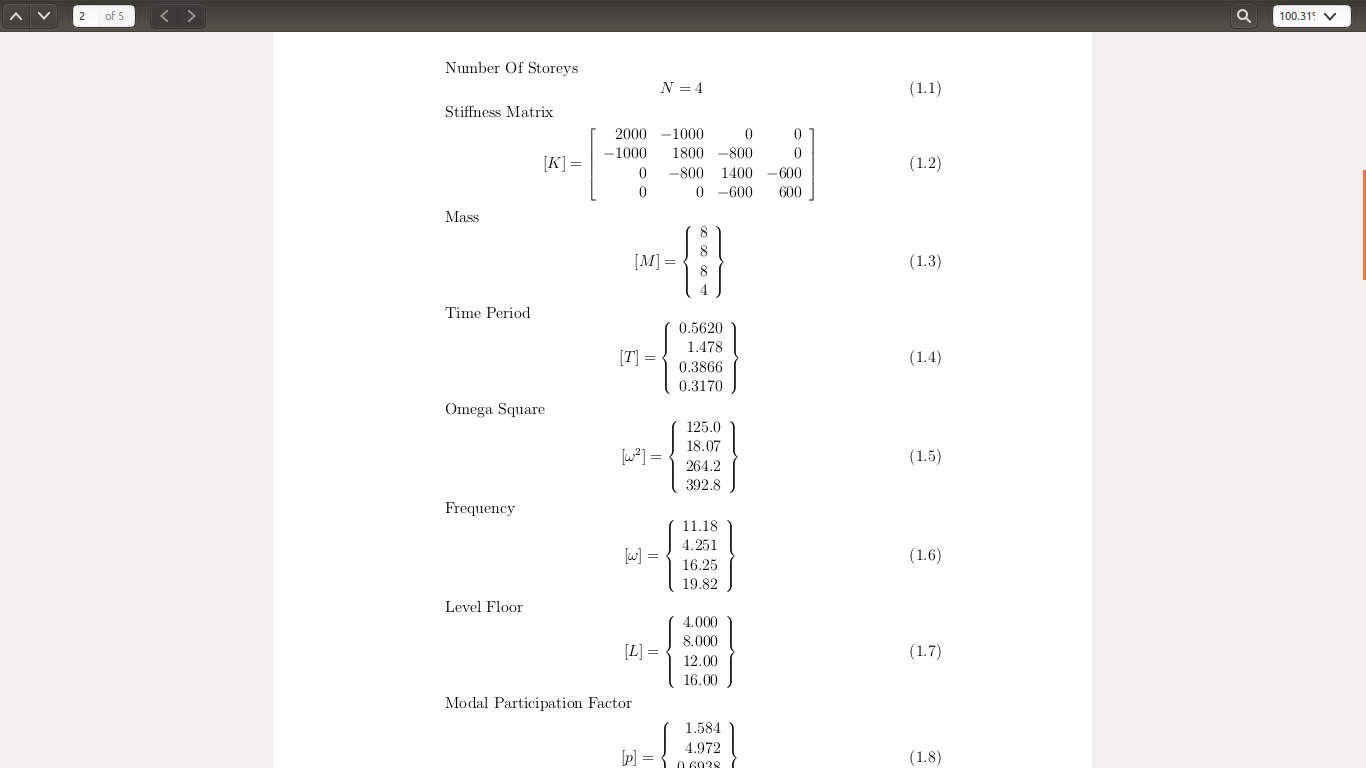
\includegraphics[scale=0.31]{images/output/7.png}
\caption{Initail values Given for Checking in PDF}
\end{figure}
\newpage
\begin{figure}[H]
\centering 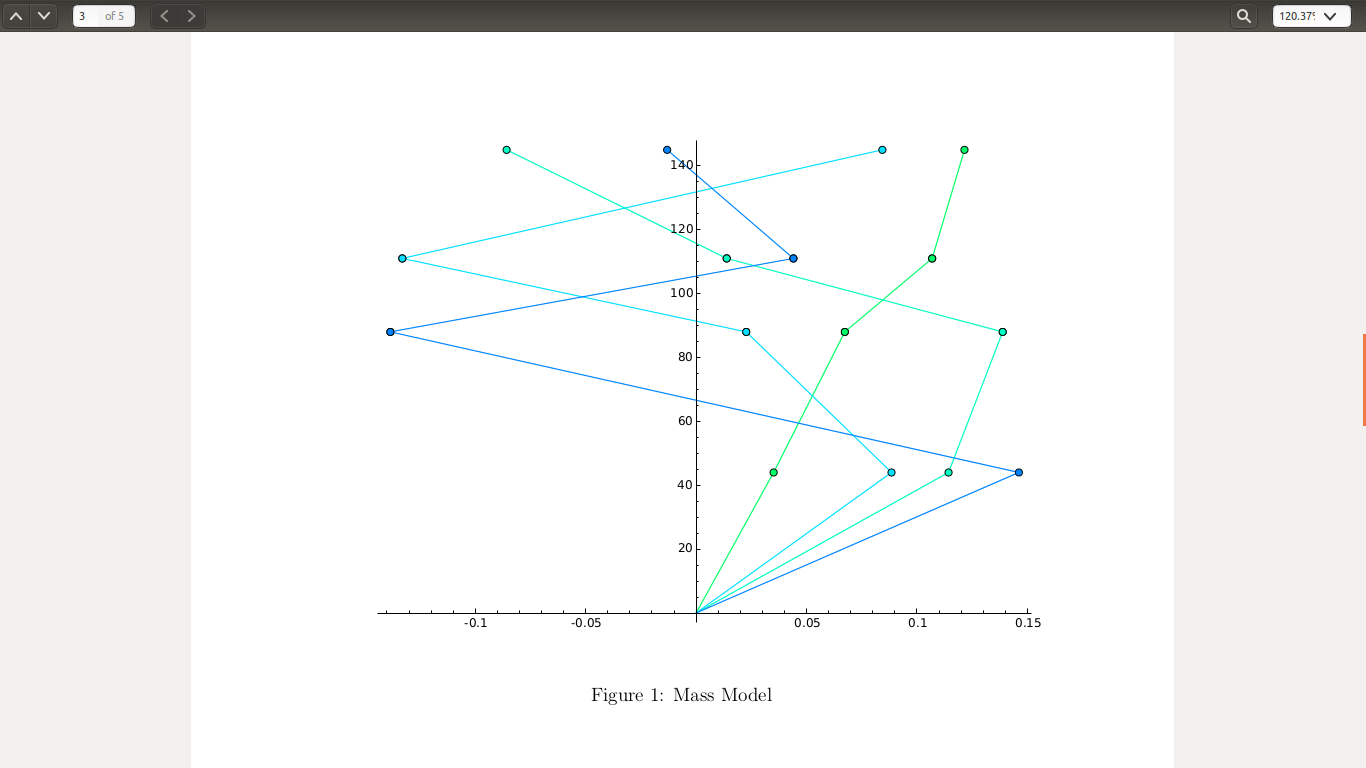
\includegraphics[scale=0.31]{images/output/8.png}
\caption{Graph Generated in PDF}
\end{figure}
\begin{figure}[H]
\centering 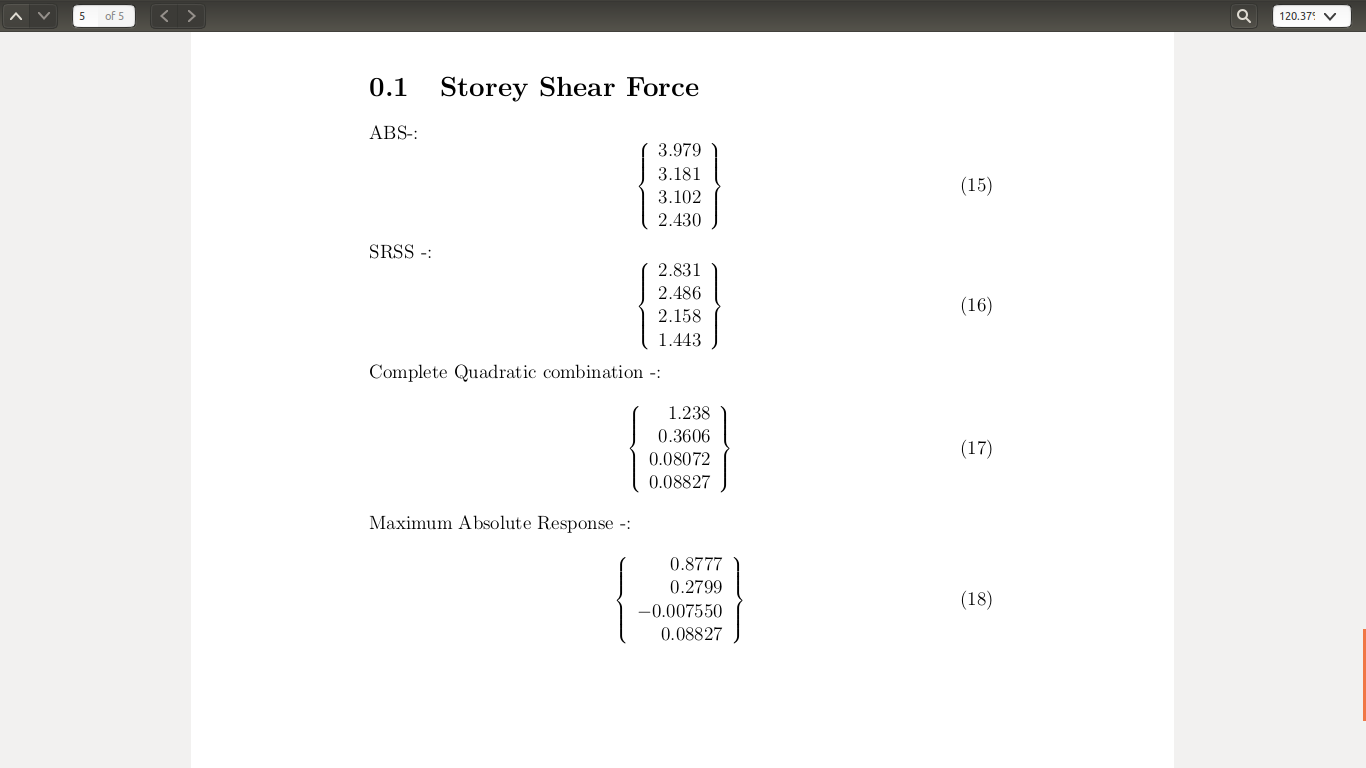
\includegraphics[scale=0.31]{images/output/9.png}
\caption{Final output in PDF}
\end{figure}
\newpage
